\documentclass[aspectratio=169,xcolor=table]{beamer}
\usetheme[style=default]{mhar-vell}
%\usepackage{helvet}
%*--------------------------------------------------
\usepackage{bibunits}  
%\setbeamertemplate{bibliography item}{[\theenumiv]}
\setbeamertemplate{bibliography item}{\insertbiblabel}
\defaultbibliography{bibliography}
%\defaultbibliographystyle{IEEEtran}
%\defaultbibliographystyle{amsalpha}
\defaultbibliographystyle{abntex2-alf}
% \bibliography{bibliography}
%\usepackage[backend=biber,style=alphabetic,citestyle=authoryear]{biblatex}
% \addbibresource{bibliography.bib}
%\usepackage{natbib}
\usepackage{bibentry}
%*--------------------------------------------------
\usepackage{epigraph}
\usepackage{graphicx}
\usepackage{multirow}
%\usepackage{enumitem}
\usepackage{array}
%\usepackage{multimedia}
\usepackage{media9}
%\usepackage{pdfpc-movie}
\usepackage{tikz}
\usepackage{circledsteps}
\usepackage{listings}
\usepackage[normalem]{ulem}
%\usepackage{Sweave}
%\usepackage{xkeyval}
%\usepackage{palatino}
%\usepackage{pgfpages}
\lstset{basicstyle=\small,breaklines=true}

%*--------------------------------------------------
\usepackage[timeinterval=1]{tdclock}
%\usepackage[font=Times,timeinterval=1, timeduration=200,resetatpages=all]{tdclock}
%\usepackage[font=Times,timeinterval=10, timeduration=2.0, timedeath=0, fillcolorwarningsecond=white!60!yellow,timewarningfirst=50,timewarningsecond=80,resetatpages=2]{tdclock}
%*--------------------------------------------------
\usepackage{url}
\usepackage{tabularx,booktabs}
\usepackage{threeparttable}
\usepackage[absolute, overlay]{textpos}
%*--------------------------------------------------
\usepackage{framed, color}
\usepackage[tikz]{bclogo}
\usepackage{spot}
\setspotlightcolor{red!50}
% %\setspotlightstyle{star, fill=red!50}
% %\setspotlightstyle{star points=7}
\usepackage{color,soul}
%\usepackage{xcolor}
\usepackage{tcolorbox}
\usepackage{xcolor}
%*--------------------------------------------------
\usepackage{amsmath}
\usepackage{xfrac}
\usepackage{units}
\usepackage{ulem}
%*-------------------------------------------------------------------------------
%\newcolumntype{C}[1]{>{\centering\arraybackslash}m{#1}}
\newcolumntype{L}[1]{>{\raggedright\let\newline\\\arraybackslash\hspace{0pt}}m{#1}}
\newcolumntype{C}[1]{>{\centering\let\newline\\\arraybackslash\hspace{0pt}}m{#1}}
\newcolumntype{R}[1]{>{\raggedleft\let\newline\\\arraybackslash\hspace{0pt}}m{#1}}
%*-------------------------------------------------------------------------------
%\pgfpagesuselayout{2 on 1}[a4paper,border shrink=5mm]
%\setbeamertemplate{note page}[plain]
%\setbeameroption{show notes on second screen=bottom}
%*-------------------------------------------------------------------------------
\setbeameroption{hide notes}
%\setbeameroption{show only notes}
%\setbeameroption{show notes on second screen=right}
\setbeamertemplate{note page}{\pagecolor{yellow!5}\insertnote}
%*-------------------------------------------------------------------------------
\title              {Docker}
\subtitle           {Como utilizar containers na robótica}
\author             {Brenda Alencar}
\email              {brenda.s1602@outlook.com}
\advisor            {Orientador: Marco A. dos Reis}
\institute          {Robótica e Sistemas Autônomos, Senai Cimatec}
\date               {Setembro de 2021}
% \ulogo        		{Template/logosenaicimatecnegativo}
% \ulogof             {Template/logosenaicimatec2020}
% \ulogoo        		{Template/rosa-logo}
% \ulistelement    	{Template/bullet-white}

%*-------------------------------------------------------------------------------
\graphicspath{{Media/pictures/}}
%*-------------------------------------------------------------------------------
\totalNoSlidesDisabled % To turn off the total number of slides in the footer. Comment this if you want the total number of slides in the footer
%*-------------------------------------------------------------------------------
\begin{document}
%*----------- COVER -------------------------------------------------------------
 \begin{frame}[t,plain]
%*----------- sound--------------------------------
    \includemedia[
        %width=1ex,
        %height=1ex,
        %activate=pageopen, 
        activate=onclick,
        deactivate=onclick,
        %passcontext,
        transparent,
        addresource=./Media/sounds/hip-hop.mp3,
        flashvars={
                    source=./Media/sounds/hip-hop.mp3
                    %&autoPlay=true
                    &autoRewind=true
                    &Play=2s
                    &repeat=always
                    %&Loop=true
        }
    ]
    {}{VPlayer.swf}
%*----------- start-page--------------------------
    \titlepage
%*----------- notes-------------------------------
    \note[item]{Notes can help you to remember important information. Turn on the notes option.}
    \note[item]{Notes can help you to remember important information. Turn on the notes option.}
\end{frame}
%-
%*----------- SECTIONS ----------------------------------------------------------
%*----------- SLIDE -------------------------------------------------------------
\begin{frame}[t]{O que é docker?} 
    \transdissolve[duration=0.5]
    É uma plataforma \textit{open source} para desenvolver, enviar e rodar aplicativos em um ambiente isolado chamado de \textit{container}.

    A tecnologia foi iniciada em 2013 pela Docker Engine para sistemas Linux, utilizando de conceitos primitivos como \textit{cgroups} e \textit{namespaces} para segregar processos.\cite{redhat}
    
    \begin{figure}
        
\includegraphics[width=.3\textwidth]{homepage-docker-logo}
    \end{figure}
%*----------- notes
    \note[item]{Notes can help you to remember important information. Turn on the notes option.}
\end{frame}
%-
%*----------- SLIDE -------------------------------------------------------------
\begin{frame}[t]{O que são \textit{containers}?} 
    \transdissolve[duration=0.5]
    \begin{columns} 
        \column{.5\textwidth}
            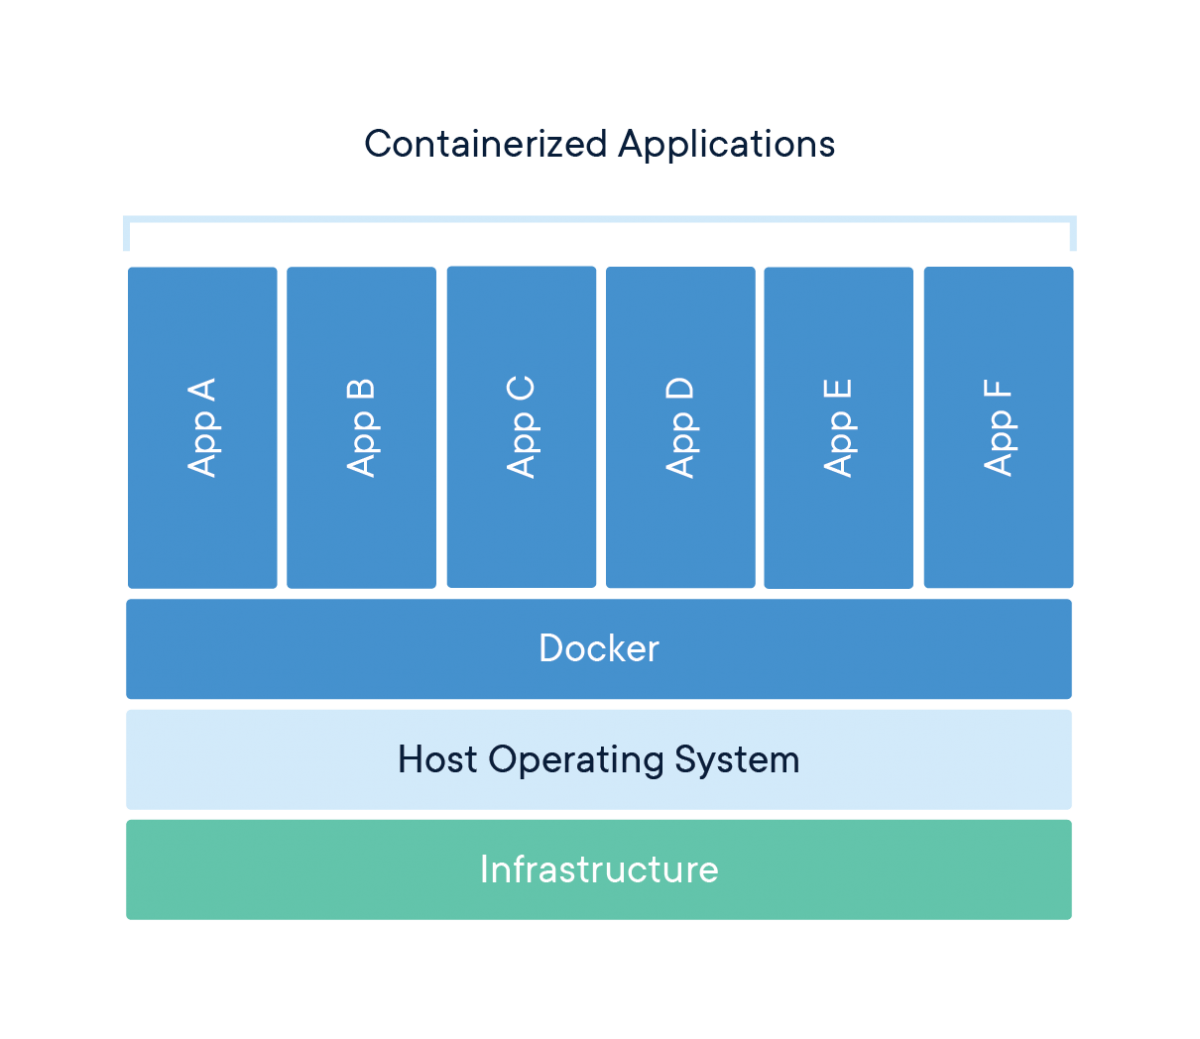
\includegraphics[width=1.1\textwidth]{container-what-is-container.png}
        \column{.5\textwidth}
            \begin{itemize}
                \item \textit{Container} é a unidade padrão do software que empacota o código e suas dependências
                \item É isolado a nível de disco, memória, processamento e rede
                \item É criado a partir de uma Imagem Docker
            \end{itemize}
          
    \end{columns}
%*----------- notes
    \note[item]{Notes can help you to remember important information. Turn on the notes option.}
\end{frame}
%-
%*----------- SLIDE -------------------------------------------------------------
\begin{frame}[t]{Arquitetura} 
    \transdissolve[duration=0.5]

    \begin{figure}
        \centering
        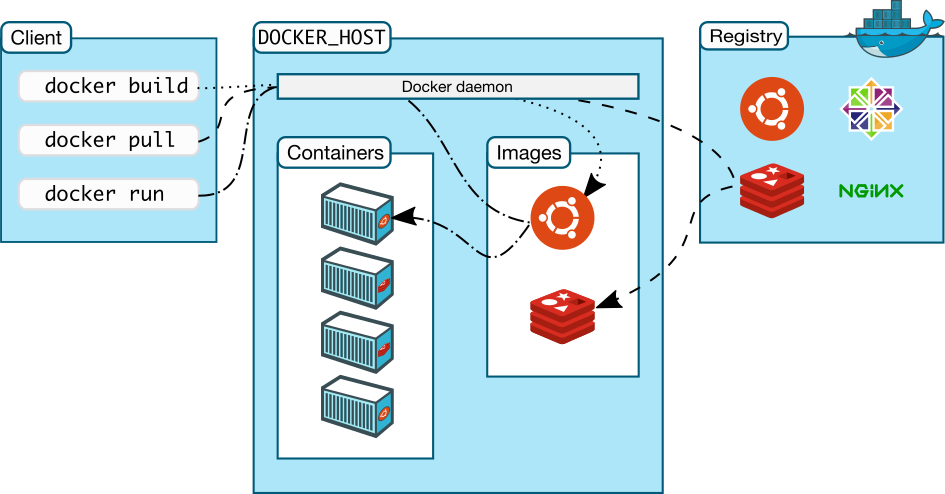
\includegraphics[width=.7\textwidth]{architecture_docker}
        \caption{\cite{docker-overview}}
    \end{figure}
%*----------- notes
    \note[item]{Notes can help you to remember important information. Turn on the notes option.}
\end{frame}
%-
%*----------- SLIDE -------------------------------------------------------------
\begin{frame}[t]{Máquina virtual x \textit{Docker}}
    São sistemas similares, utilizam virtualização para executar um programa como se fosse uma máquina física    \cite{dock}
    \begin{columns} 
        \column{.5\textwidth}
            \begin{center}
                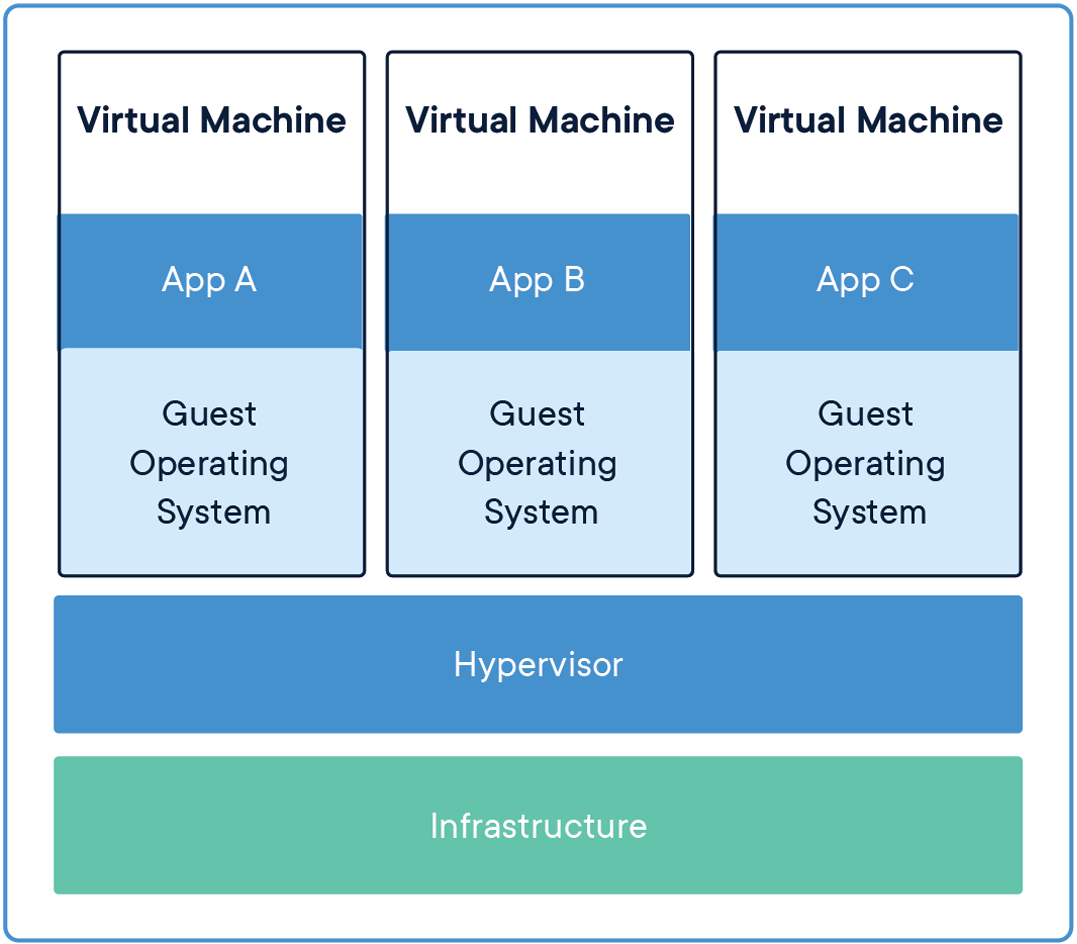
\includegraphics[width=0.7\textwidth]{vm1}
            \end{center}
        \column{.5\textwidth}
            \begin{center}
                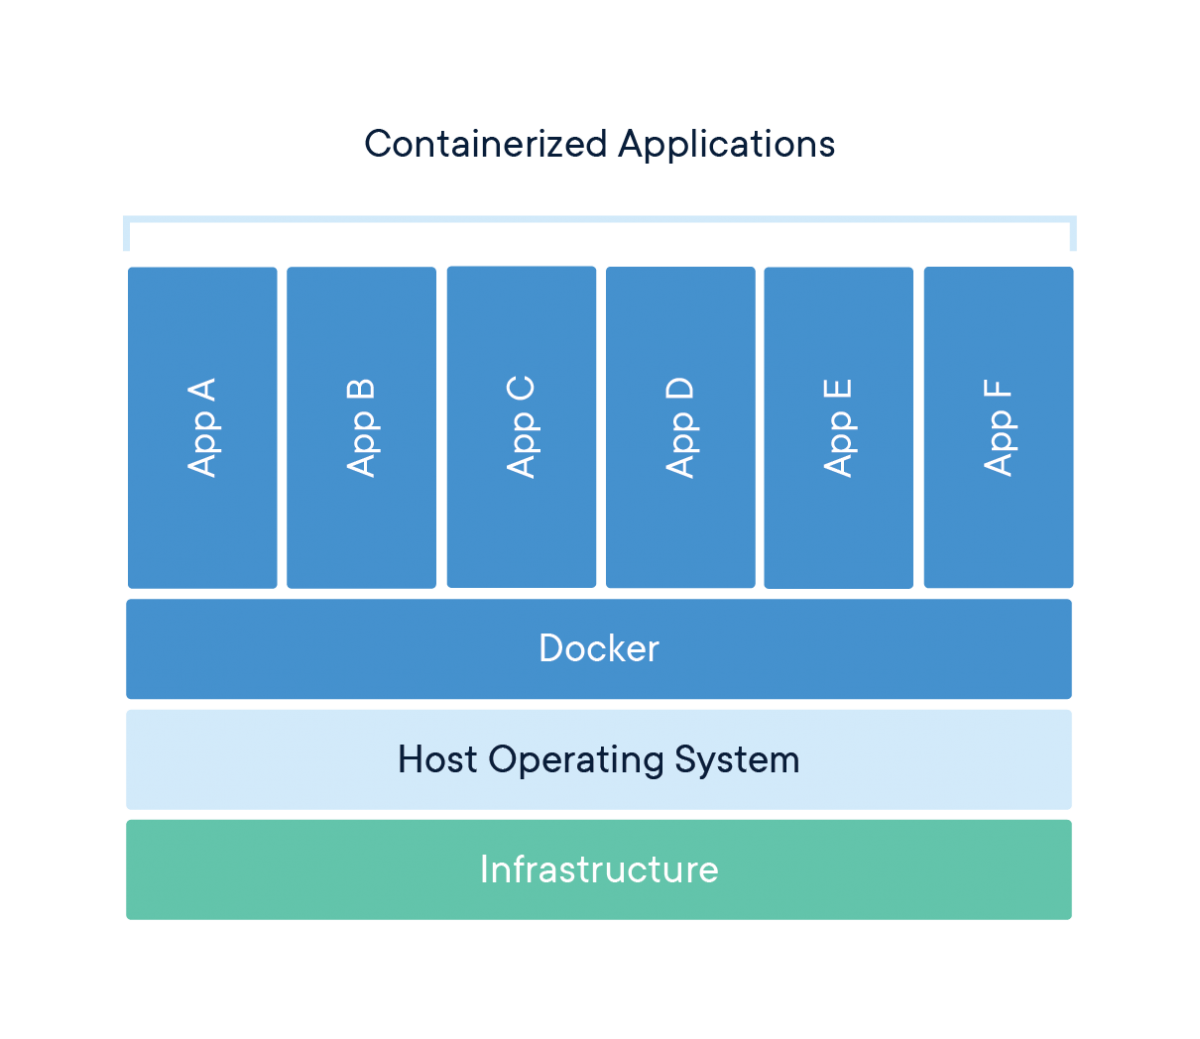
\includegraphics[width=.95\textwidth]{container-what-is-container}
            \end{center}
    \end{columns}
%*----------- notes
    \note[item]{Notes can help you to remember important information. Turn on the notes option.}
\end{frame}

%*----------- SLIDE -------------------------------------------------------------
\begin{frame}[fragile, t]{Primeiros passos}
    \begin{enumerate}
        \item Instalar Docker
            \href{https://docs.docker.com/engine/install/ubuntu/}{Instalação para Ubuntu}
        \item Hello world
        \begin{lstlisting}
            $ sudo docker run hello-world
        \end{lstlisting}
        \item Instalar extensão para VSCode
            ID: ms-azuretools.vscode-docker
    \end{enumerate}
%*----------- notes
    \note[item]{Notes can help you to remember important information. Turn on the notes option.}
\end{frame}
%-
%*----------- SLIDE -------------------------------------------------------------
\begin{frame}[fragile, t]{Comandos básicos}

    \begin{lstlisting}
        # Extrair/enviar uma imagem para um repositorio
        $ docker pull ubuntu:bionic
        $ docker push ubuntu:bionic25

        # Cria e inicializa um container gravavel 
        $ docker run [OPTIONS] ubuntu:bionic bash

        # Pausa/Inicia um ou mais containers
        $ docker stop NAME
        $ docker start NAME

        # Executa um comando em um container em execucao
        $ docker exec -ti NAME 

    \end{lstlisting}
%*----------- notes
    \note[item]{Notes can help you to remember important information. Turn on the notes option.}
\end{frame}
%-
%*----------- SLIDE -------------------------------------------------------------
\begin{frame}[fragile, t]{Comandos básicos}

    \begin{lstlisting}
        # Mostra as imagens criadas,tamanho,repositorio,tag 
        $ docker image ls

        # Lista containers
        $ docker ps [OPTIONS]

        # Para fechar um terminal integrado com o container
          "Ctrl+D"

        # Remove um ou mais containers/imagens
        $ docker rm [OPTIONS] NAME 
        $ docker rmi [OPTIONS] NAME_IMAGE 


    \end{lstlisting}
%*----------- notes
    \note[item]{Notes can help you to remember important information. Turn on the notes option.}
\end{frame}
%-
%*----------- SLIDE -------------------------------------------------------------
\begin{frame}[fragile, t]{Docker+ROS}
    1- Iniciar um \textit{container} com a imagem do ros que deseja; 
    
    2- Iniciar um \textit{container} com a imagem do Ubuntu necessário para o ros e então \href{http://wiki.ros.org/kinetic/Installation/Ubuntu}{instalar} o ros normalmente
    \begin{lstlisting}
        docker pull ubuntu:xenial
        docker run --name teste -ti ubuntu:xenial  bash
        apt-get update && apt-get install -y lsb-release wget && apt-get clean all  

        # seguir com os passos da instalação do ros

    \end{lstlisting}
%*----------- notes
    \note[item]{Notes can help you to remember important information. Turn on the notes option.}
\end{frame}
%-
%*----------- SLIDE -------------------------------------------------------------
\begin{frame}[fragile, t]{GUI's+ROS}
    # explicar a forma mais segura
    \begin{lstlisting}
        docker run -it \
            --env="DISPLAY" \
            --env="QT_X11_NO_MITSHM=1" \
            --volume="/tmp/.X11-unix:/tmp/.X11-unix:rw" \
            ubuntu:xenial \
        export containerId=$(docker ps -l -q)

        xhost +local:`docker inspect --format='{{ .Config.Hostname }}' $containerId`
        docker start $containerId

    \end{lstlisting}
%*----------- notes
    \note[item]{Notes can help you to remember important information. Turn on the notes option.}
\end{frame}
%-
\input{Sections/04-results}
%----------------------------------------------------SLIDE------------------
 \begin{frame}[t, allowframebreaks]{References}
 %\frametitle{References}
%\begin{frame}{Reference}
    %\transboxin[duration=1,direction=30]

    % \begin{bibunit}[plain]
    % %\cite{kanakia2012}
    % %\cite{agostini2007}
    % %\cite{azuma1997survey}
    % \cite{Buss2005}
  
    % \putbib
    % \end{bibunit}
  
    %\bibliographystyle{IEEEtran}
    %\bibliographystyle{IEEEtranS}
    %\bibliographystyle{IEEEbib}
    \bibliographystyle{abntex2-alf}
    %\bibliographystyle{abntex2-num}
    %\bibliographystyle{abnt-alf}
    \bibliography{bibliography} 
    %\putbib

%*----------- notes
    %\note[item]{Notes can help you to remember important information. Turn on the notes option.}
\end{frame}
%
%-
%*----------- SLIDE-BACKUP ------------------------------------------------------
% \backupbegin
% %
% \begin{frame}{Backup}
%     Test
% %*----------- notes-------------------------------
% \note{Notes can help you to remember important information. Turn on the notes option.}
% \end{frame}
% %-
% \backupend
% %-
%*----------- QUESTIONS ---------------------------------------------------------
\begin{frame}[c,plain]
    \lastpage{
        \begin{center}   
            {\usebeamerfont{title} Questions?}\\[3ex] 
            %\hspace{1.5cm} 
            brenda.s1602@outlook.com
        \end{center}
    }
    
%*----------- notes---------------------------------
    \note[item]{Notes can help you to remember important information. Turn on the notes option.}
\end{frame}
%*-------------------------------------------------------------------------------
\end{document}